\section{二次函数与几何}



\subsection{二次函数的几何变换}

\subsubsection*{平移}
还记得平移运动吗?简单回顾:平移是全等的几何变换(平移前和平移后的图形全等),平移具有交换性(比如一个正方形先向上平移3个单位再向左平移3个单位,如果颠倒顺序,最终位置相同)和可逆性(平移后可以通过反向平移回到原位置).
\par
对二次函数平移其实就是\textbf{对二次函数的顶点平移},进行任何平移操作前需要先把二次函数化为顶点式以方便操作.
\par
假设有\(y=a(x-h)^2\),若\(h>0\)则函数向左平移,若\(h<0\)则函数向右平移,都是平移\(|h|\)个单位;假设有\(y=ax^2+k\),若\(k>0\)则函数向上平移,若\(k<0\)则函数向下平移,都是平移\(|k|\)个单位.两者一起进行就是顶点式\(y=a(x-h)^2+k\).
\par
\begin{example}抛物线\( l_1 \)是由抛物线\( l_2 \)向下平移3个单位长度,再向左平移2个单位长度得到的,已知抛物线\( l_1 \)的解析式为\( y=2(x-2)^2+3 \),则抛物线\( l_2 \)的解析式为(\hspace{3.5em})

\begin{enumerate}[label=\Alph*.]
    \item \( y=2(x-4)^2+6 \)
    \item \( y=2(x-2)^2 \)
    \item \( y=2x^2+6 \)
    \item \( y=2x^2 \)
\end{enumerate}
\end{example}
\begin{solution}
    分析:因为1由2向下平移3个单位再向左平移2个单位,题目已知1求2,只需对1进行反向操作,即向右平移2个单位再向上平移3单位,经过计算A正确.
\end{solution}
以上是抛物线沿坐标轴方向平移的例子,如果沿斜向(即直线)平移呢?这时候只要知道平移的距离和直线的解析式,过移动后的顶点做垂线,垂直于坐标轴,就能\textbf{构造一个直角三角形}.根据直线解析式,\textbf{设移动后顶点的坐标},顶点的横纵坐标值就是三角形直角边的长,最后通过\textbf{勾股定理}就能得出移动后顶点的坐标.
\begin{example}
    将抛物线 \( y = x^2 \) 沿直线 \( y = 3x \) 方向移动 \(\sqrt{10}\) 个单位长度,若移动后抛物线的顶点在第一象限,则移动后抛物线的解析式是\underline{\hspace{4em}}。
\end{example}
\begin{solution}
    分析:该二次函数沿一条直线移动,没有指定移动的方向,但题目要求移动后二次函数的顶点在第一象限,因为该直线(正比例函数)的斜率为\(3>0\),\(x>0\)时\(y\)随\(x\)的增大而增大,所以只有在二次函数往右上方移动时才符合题意(可以画草图辅助理解,如图\ref{fig:move1}),此时根据正比例函数可以设移动后的坐标为\((m,3m)\),再作\(BA\)垂直于\(x\)轴,原点为点\(C\),移动后的定点坐标为\(B\),\(BA=3m,CA=m,CB=\sqrt{10}\),利用勾股定理即可求出移动后的顶点坐标,根据顶点坐标列成顶点式再化为一般式即可.
    \par
    \begin{figure}[h]
        \centering
    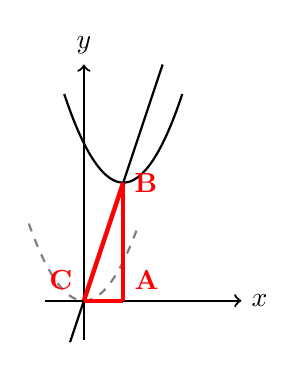
\begin{tikzpicture}[scale=0.5]
    % 绘制坐标系
                                        \draw[->, thick] (-1,0) -- (4,0) node[right] {$x$}; % x轴
                                        \draw[->, thick] (0,-1) -- (0,6) node[above] {$y$}; % y轴
                                        \draw[domain=-1.4:1.4, smooth, dashed, thick, gray] plot (\x, {\x*\x}); % 标注函数
                                        \draw[domain=-0.35:2, smooth, thick] plot (\x, {\x*3}); % 标注函数
                                        \draw[domain=-0.5:2.5, smooth, thick, black] plot (\x, {(\x - 1)^2 + 3}); % 标注函数
                                        \draw[red, ultra thick] (0,0) node[above left] {$\textbf{C}$} -- (1,3) node[right] {$\textbf{B}$};
                                        \draw[red, ultra thick] (1,0) node[above right] {$\textbf{A}$} -- (1,3);
                                        \draw[red, ultra thick] (0,0) -- (1,0);
    \end{tikzpicture}
    \caption{}
        \label{fig:move1}
    \end{figure}
\end{solution}


\noindent
\begin{minipage}{1\linewidth}
\begin{wrapfigure}{r}{3cm}
    \vspace{-2cm}
    \centering
    \begin{minipage}{1\linewidth}
    \centering
        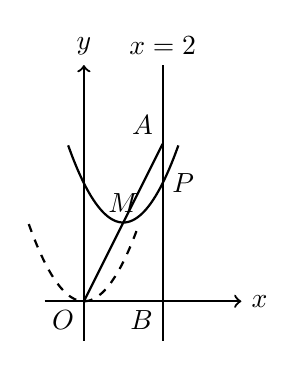
\begin{tikzpicture}[scale=0.5] % 整体缩放
                                        % 绘制坐标系
                                        \draw[->, thick] (-1,0) -- (4,0) node[right] {$x$}; % x轴
                                        \draw[->, thick] (0,-1) -- (0,6) node[above] {$y$}; % y轴
                                        % 标注原点 O
                                        \node at (0,0) [below left] {$O$};
                                        % 绘制点 A(2,4)
                                        \filldraw (2,4) circle (0pt) node[above left] {$A$};
                                        % 绘制直线 x=2(虚线)
                                        \draw[thick] (2,-1) -- (2,6) node[above] {$x=2$};
                                        % 绘制点 B(2,0)
                                        \filldraw (2,0) circle (0pt) node[below left] {$B$};
                                        % 绘制直线 OA(实线)
                                        \draw[thick] (0,0) -- (2,4) node[midway, above left, black] {}; % 不额外标注
                                        % 绘制初始二次函数 y=x^2(虚线,示意原始位置)
                                        \draw[domain=-1.4:1.4, smooth, dashed, thick] plot (\x, {\x*\x}); % 标注函数
                                        % 绘制平移后的二次函数(示例:顶点 M 在 (1,2) 处)
                                        % 函数解析式:y = (x-1)^2 + 2 = x^2 - 2x + 3
                                        \draw[domain=-0.4:2.4, smooth, thick] plot (\x, {(\x-1)^2 + 2}); % 标注
                                        % 标注顶点 M(1,2)
                                        \filldraw (1,2) circle (0pt) node[above] {$M$};
                                        % 标注点 P(2,3)(二次函数与 x=2 的交点)
                                        \filldraw (2,3) circle (0pt) node[right] {$P$};
                                        
                                        \end{tikzpicture}
                                        \par
    题图1
    \end{minipage}
    \end{wrapfigure}
\begin{minipage}{1\linewidth}
\begin{exercise}
    \small
    \setlength{\parindent}{0pt} % 取消段落缩进
    \setlength{\columnseprule}{0.01pt}
    \begin{multicols}{2}
    (1)如题图1,在平面直角坐标系中,已知点 \( A \) 坐标为 \((2,4)\),直线 \( x=2 \) 与 \( x \) 轴相交于点 \( B \),连接 \( OA \),二次函数 \( y=x^2 \) 图象从点 \( O \) 沿 \( OA \) 方向平移,与直线 \( x=2 \) 交于点 \( P \),顶点 \( M \) 到 \( A \) 点时停止移动。
    %\begin{figure}[h]
        %\centering
        
    %\end{figure}
    \begin{enumerate}
        \item 求线段 \( OA \) 所在直线的函数解析式.
        \item 设二次函数顶点 \( M \) 的横坐标为 \( m \),当 \( m \) 为何值时,线段 \( PB \) 最短,并求出二次函数的解析式.
        \item 当线段 \( PB \) 最短时,二次函数的图象能否过点 \( Q(a,a-1) \) ? 若能,求出 \( a \) 的值;若不能,请说明理由.
    \end{enumerate}




    (2)已知抛物线 \( y = ax^2 - 2ax - 8 \ (a \neq 0) \),若将该函数先向左平移 1 个单位,再向上平移 9 个单位,顶点恰好落在原点上。

    \begin{enumerate}
        \item 求抛物线的函数解析式和顶点坐标;
        \item 若有一直线 \( l \) 与抛物线交于点 \( A(-3, m) \),\( B(n, 16) \),且 \( n > 0 \)。若点 \( P \) 在抛物线上且在直线 \( l \) 下方,且点 \( P \) 不与点 \( A, B \) 重合,分别求出点 \( P \) 横坐标与纵坐标的取值范围。
    \end{enumerate}
    
    \end{multicols}
    \end{exercise}
    \end{minipage}
\end{minipage}
    










\subsubsection*{轴对称}

还记得轴对称吗?简单回顾:轴对称是全等的几何变换(对称前后的图形全等),轴对称具有自反性(一个图形关于某直线对称后,再对同一条直线对称一次,图形就会回到原来的位置)。例如,一个等腰三角形沿着它的高线对称后,再对同一条高线对称一次,就恢复成原来的等腰三角形.此外,对称轴上的任意一点到图形对应点的距离相等.
\par

\noindent
\begin{minipage}{1\linewidth}
    \begin{wrapfigure}{r}{3cm}
    \vspace{-1cm}
    \hspace{-1.4cm}
    \centering
    \begin{center}
    \centering
        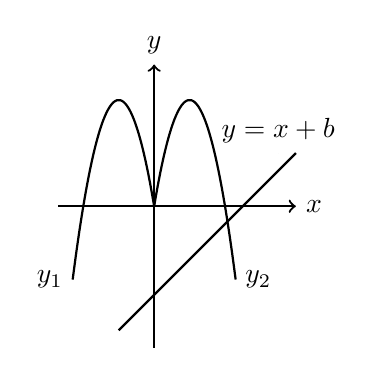
\begin{tikzpicture}[
            scale=0.45,
            declare function={
                func(\x) = -3*(\x+1)^2 + 3;
                func2(\x) = -3*(-\x+1)^2 + 3;
                func3(\x) = \x -2.5;
            }
        ]
            \draw[->, thick] (-2.7, 0) -- (4, 0) node[right] {$x$};
            \draw[->, thick] (0, -4) -- (0, 4) node[above] {$y$};
        
            \draw[domain=-2.3:0, smooth, thick, variable=\x] plot ({\x}, {func(\x)});
            \pgfmathsetmacro{\xleft}{-2.3}
            \pgfmathsetmacro{\yleft}{func(\xleft)}
            % 在左侧端点右侧添加y₁标记
            \filldraw (\xleft,\yleft) circle (0pt);
            \node[left] at (\xleft,\yleft) {$y_1$};
        
            
            \draw[domain=0:2.3, smooth, thick, variable=\x] plot ({\x}, {func2(\x)});
            \pgfmathsetmacro{\xleft}{2.3}
            \pgfmathsetmacro{\yleft}{func2(\xleft)}
            % 在左侧端点右侧添加y₁标记
            \filldraw (\xleft,\yleft) circle (0pt);
            \node[right] at (\xleft,\yleft) {$y_2$};
            
            \draw[domain=-1:4, smooth, thick, variable=\x] plot ({\x}, {func3(\x)});
            \pgfmathsetmacro{\xleft}{3.5}
            \pgfmathsetmacro{\yleft}{func3(\xleft)+0.5}
            % 在左侧端点右侧添加y₁标记
            \filldraw (\xleft,\yleft) circle (0pt);
            \node[above] at (\xleft,\yleft) {$y=x+b$};
            
        \end{tikzpicture}
        例题图
    \end{center}
    \vspace{0.7cm}
        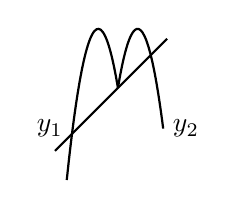
\begin{tikzpicture}[
            scale=0.25,
            declare function={
                func(\x) = -3*(\x+1)^2 + 3;
                func2(\x) = -3*(-\x+1)^2 + 3;
                func3(\x) = \x;
            }
        ]
            \draw[domain=-2.6:0, smooth, thick, variable=\x] plot ({\x}, {func(\x)});
            \pgfmathsetmacro{\xleft}{-2.3}
            \pgfmathsetmacro{\yleft}{func(\xleft)}
            % 在左侧端点右侧添加y₁标记
            \filldraw (\xleft,\yleft) circle (0pt);
            \node[left] at (\xleft,\yleft) {$y_1$};
        
            
            \draw[domain=0:2.3, smooth, thick, variable=\x] plot ({\x}, {func2(\x)});
            \pgfmathsetmacro{\xleft}{2.3}
            \pgfmathsetmacro{\yleft}{func2(\xleft)}
            % 在左侧端点右侧添加y₁标记
            \filldraw (\xleft,\yleft) circle (0pt);
            \node[right] at (\xleft,\yleft) {$y_2$};
            
            \draw[domain=-3.2:2.5, smooth, thick, variable=\x] plot ({\x}, {func3(\x)});
            
        \end{tikzpicture}
        
        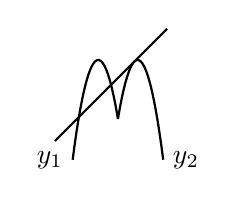
\begin{tikzpicture}[
            scale=0.25,
            declare function={
                func(\x) = -3*(\x+1)^2 + 3;
                func2(\x) = -3*(-\x+1)^2 + 3;
                func3(\x) = \x + 25/12;
            }
        ]
            \draw[domain=-2.3:0, smooth, thick, variable=\x] plot ({\x}, {func(\x)});
            \pgfmathsetmacro{\xleft}{-2.3}
            \pgfmathsetmacro{\yleft}{func(\xleft)}
            % 在左侧端点右侧添加y₁标记
            \filldraw (\xleft,\yleft) circle (0pt);
            \node[left] at (\xleft,\yleft) {$y_1$};
        
            
            \draw[domain=0:2.3, smooth, thick, variable=\x] plot ({\x}, {func2(\x)});
            \pgfmathsetmacro{\xleft}{2.3}
            \pgfmathsetmacro{\yleft}{func2(\xleft)}
            % 在左侧端点右侧添加y₁标记
            \filldraw (\xleft,\yleft) circle (0pt);
            \node[right] at (\xleft,\yleft) {$y_2$};
            
            \draw[domain=-3.2:2.5, smooth, thick, variable=\x] plot ({\x}, {func3(\x)});
            
        \end{tikzpicture}
    \end{wrapfigure}

    \begin{example}
        
        如右图,函数 \( y_1 = -a(x+1)^2 + 3 \) (\( x < 0 \)) 的图象过原点,将其沿 \( y \) 轴翻折,得到函数 \( y_2 \) 的图象,把函数 \( y_1 \) 与 \( y_2 \) 的图象合并后称为函数 \( L \) 的图象.
        
        \begin{enumerate}
            \item \( a \) 的值为\underline{\hspace{3.5em}};函数 \( y_2 \) 的解析式为\underline{\hspace{3.5em}}(注明 \( x \) 的取值范围);
            \item 当直线 \( y = x + b \) 与函数 \( L \) 的图象有 3 个公共点时,求 \( b \) 的值.
        \end{enumerate}
        
    \end{example}

    \begin{solution}
    \begin{enumerate}
    \item 分析:第一空要求\(a\),观察解析式只有一个参数,所以只需要找出一个点就可以求\(y_1\)解析式和\(a\)的值,阅读题目得知\(y_1\)过原点即\((0,0)\),将\(x=0,y=0\)代入原解析式即可求出\(a\)的值,第二空要求\(y_2\)的值,即求将\(y_1\)沿\(y\)轴翻折的解析式,只需改变\(y_1\)解析式的\(x\)为\(-x\)即可,最后注意标注自变量的取值范围.
    \item 分析:画草图分析(如右两小图),上下平移直线\(y=x+b\)发现只有两种情况与函数L有三个公共点,第一种:已知函数L过原点,当直线\(y=x+b\)也过原点(即\(b=0\)时),满足条件,第二种:直线\(y=x+b\)与函数L的\(y_2\)部分只有一个交点(即相切)的时候符合条件,此时要计算参数\(b\)的值需要结合前面学习抛物线交点相关问题的知识点,抓住直线与抛物线\(y_2\)只有一个交点这一条件,将二次函数\(y_2\)与一次函数\(y=x+b\)的解析式联立,得到一个含参数\(b\)的一元二次方程,因为只有一个交点所以该方程的判别式等于0,即\(\Delta=0\),依据判别式列出一个含参数\(b\)的方程,解方程就能得到第二种情况\(b\)的值.
    \end{enumerate}
    \end{solution}

\end{minipage}






\subsection{设参思想(点参、线参)}

在学习一次函数时,我们就接触过设参,设参思想是处理二次函数综合问题的核心代数化策略,其本质是通过引入辅助变量(称为参数)将几何动态问题转化为可计算的代数模型。当抛物线上的点$P$位置变化时,设其横坐标为参数$t$,根据二次函数解析式 $y = ax^2 + bx + c$,点$P$的纵坐标可直接用含$t$的代数式表示为:
\[
y = a \cdot t^2 + b \cdot t + c
\]
此时点$P$的完整坐标可记为:
\[
P(t,\  at^2 + bt + c)
\].该操作的数学意义在于:
\begin{itemize}
    \item 将连续运动的点转化为连续变化的参数.
    \item 通过特定条件控制参数的取值,用于描述几何关系
\end{itemize}

\subsection{二次函数与\textbf{线段}}

\subsubsection*{线段值}
\noindent
\begin{minipage}{1\linewidth}
    \begin{wrapfigure}{r}{3cm}
    \vspace{-2cm}
    \hspace{-1.4cm}
    \centering
    \begin{center}
    \centering
        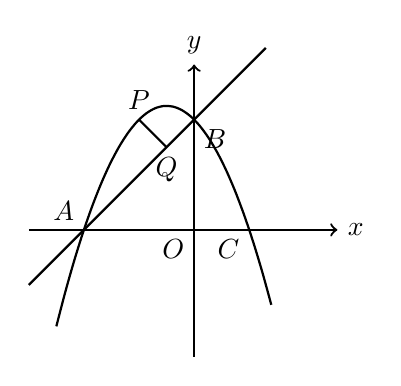
\begin{tikzpicture}[
            scale=0.7,
            declare function={
                func(\x) = -(\x+2)*(\x-1);
                func2(\x) = \x +2;
            }
        ]
            \draw[->, thick] (-3, 0) -- (2.6, 0) node[right] {$x$};
            \draw[->, thick] (0, -2.3) -- (0, 3) node[above] {$y$};

            \filldraw (-1,2) circle (0pt) node[above] {$P$};

            \filldraw (-2,0) circle (0pt) node[above left] {$A$};
            \filldraw (0,2) circle (0pt) node[below right] {$B$};
            \filldraw (1,0) circle (0pt) node[below left] {$C$};
            \filldraw (0,0) circle (0pt) node[below left] {$O$};
            \draw[black, thick] (-1,2) -- (-0.5,1.5) node[below] {$Q$};
        
            \draw[domain=-2.5:1.4, smooth, thick, variable=\x] plot ({\x}, {func(\x)});
            
            \draw[domain=-3:1.3, smooth, thick, variable=\x] plot ({\x}, {func2(\x)});
            
        \end{tikzpicture}
        例题图
        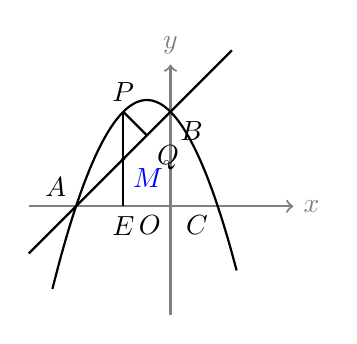
\begin{tikzpicture}[
            scale=0.6,
            declare function={
                func(\x) = -(\x+2)*(\x-1);
                func2(\x) = \x +2;
            }
        ]
            \draw[->, thick, gray] (-3, 0) -- (2.6, 0) node[right] {$x$};
            \draw[->, thick, gray] (0, -2.3) -- (0, 3) node[above] {$y$};

            \filldraw (-1,2) circle (0pt) node[above] {$P$};

            \filldraw (-2,0) circle (0pt) node[above left] {$A$};
            \filldraw (0,2) circle (0pt) node[below right] {$B$};
            \filldraw (1,0) circle (0pt) node[below left] {$C$};
            \filldraw (0,0) circle (0pt) node[below left] {$O$};
            \filldraw[blue] (-1,1) circle (1pt) node[below right, blue] {$M$};

            
            \draw[black, thick] (-1,2) -- (-0.5,1.5) node[below right] {$Q$};
            \draw[black, thick] (-1,2) -- (-1,0) node[below] {$E$};
            \draw[domain=-2.5:1.4, smooth, thick, variable=\x] plot ({\x}, {func(\x)});
            
            \draw[domain=-3:1.3, smooth, thick, variable=\x] plot ({\x}, {func2(\x)});
            
        \end{tikzpicture}
    \end{center}
    
    \end{wrapfigure}

    \begin{example}
        
        如图,在平面直角坐标系中,直线 \( y = x + 2 \) 与坐标轴交于 \( A \),\( B \) 两点,点 \( A \) 在 \( x \) 轴上,点 \( B \) 在 \( y \) 轴上,点 \( C \) 的坐标为(1,0),抛物线 \( y = -x^2-x + 2 \) 经过点 \( A \),\( B \),\( C \).若点 \( P \) 是抛物线上一动点,且在直线 \( AB \) 上方,过点 \( P \) 作 \( AB \) 的垂线段,垂足为点 \( Q \)。当 \( PQ = \dfrac{\sqrt{2}}{2} \) 时,求点 \( P \) 的坐标.
        
    \end{example}

    \begin{solution}
    分析:由题可知\(PQ=\dfrac{\sqrt{2}}{2}\)和\(PQ\perp AB\)可以联想到需要想利用等腰直角三角形的边长比\(1:1:\sqrt{2}\),此时需要构造等腰直角三角形.就题目所给的条件来看无法构造两等边,所以考虑构造等角,由题意可知\(AO=OB,\angle AOB=90^\circ\),所以\(\triangle AOB\)是等腰直角三角形,所以\(\angle BAO=45^\circ\).由此可以做\(PE\perp x\)轴,易知\(\triangle AEM\)是等腰直角三角形,还可以知道\(\angle AEM=\angle PQM\),利用八字模型易知\(\triangle PQM\)是等腰直角三角形.构造等腰直角三角形完成.由三边比关系可以算出\(PM=1\)
    \par
    抓住\(PM=1\)这一条件,观察图像,发现\(PM=PE-ME=|y_P-y_M|=1\),可以设点\(P\)和点\(P\)的参数,代入该关系式,可以解出\(P\)横坐标,再讲\(P\)横坐标代回点\(P\)的纵坐标即可求出\(P\)的坐标
    \end{solution}

\end{minipage}

\subsubsection*{线段关系}

\subsubsection*{线段最值}

\subsection{二次函数与\textbf{面积}}

\subsubsection*{面积公式与割补}

\subsubsection*{铅锤法}

\subsubsection*{转化法}

\subsection{二次函数与\textbf{角度}}

\subsubsection*{角度定值或范围}

\subsubsection*{角度数量关系}

\subsection{二次函数与\textbf{特殊几何图形}}

\subsubsection*{特殊三角形}

\subsubsection*{特殊四边形}